\documentclass{article}

\def\subj {CSCE}
\def\npart {121}
\def\nterm {Fall}
\def\nyear {2018}
\def\ncourse {Intro to Programming Design and Concepts}



\input{header}

\setlength\parindent{0pt}

\begin{document}
\maketitle
%{\small
%  \noindent\textbf{Heat Equation}\\
%  Conduction of Heat in a 1-Dimensional rod, boundary conditions, equilibrium temperature distribution, heat condition in 2 or 3 dimensions.\hspace*{\fill} [1]
%
%  \vspace{10pt}
%  \noindent\textbf{Method of Separation of Variables}\\
%  Linearity, heat equation with zero temperatures at finite ends, orthogonality of functions, Laplace's equation; solutions and qualitative properties.\hspace*{\fill} [2]
%
%  \vspace{10pt}
%  \noindent\textbf{Fourier Series}\\
%  Statement of Convergence Theorem, Fourier cosine and sine series, term-by-term differentiation of Fourier series, term-by-term integration of Fourier series, complex form of Fourier series.\hspace*{\fill} [3]
%
%  \vspace{10pt}
%  \noindent\textbf{Wave Equation}\\
%  Vertically vibrating string, boundary conditions, vibrating string with fixed ends, vibrating membrane, reflection and refraction of electromagnetic and acoustic sound waves.\hspace*{\fill} [4]
%  
%  \vspace{10pt}
%  \noindent\textbf{The Method of Characteristics for Linear and Quasilinear
%  	Wave Equations}\\
%  Characteristics for first order wave equations, method of characteristics for first order PDEs, one-dimensional wave equation, a vibrating string of fixed length, many quasilinear PDEs, semi-infinite strings and reflections. \hspace*{\fill} [12]
%  
%  \vspace{10pt}
%  \noindent\textbf{Fourier Transform Solutions of Partial
%  	Differential Equations}\\
%  Heat equation on an infinite domain, Fourier transform pair, inverse Fourier transform, convolution theorem.\hspace*{\fill} [10]
%
%  \vspace{10pt}
%  \noindent\textbf{Green’s Functions for Time-Independent Problems}\\
%  Green's functions for boundary value problems for ODEs, method of eigenvalue expansion, nonhomogeneous boundary conditions.\hspace*{\fill} [9]}

\tableofcontents

	\section{Computer Architecture and Compilation Process}
	
	\subsection{Basic Architecture}
	
	The majority of modern computers are built using the Von Neumann architecture, where the CPU is where the computational power resides, the memory unit stores program code and data, and the two are connected by a ``bus."\\
	
	During each computation cycle, the machine retrieves the next instruction from the memory unit. Then subsequently executes the computation associated with the retrieved instruction. This process is repeated until the machine is told to halt.
	
	\subsection{Memory}
	
	The smallest unit of memory is the \textit{bit}, which can be one of two states.\\
	
	Computers use transistor circuits known as `flip-flops' to store bits. It can either be on (1) or off (0). \\
	
	The byte (8 bits) is the smallest accessable unit of memory in a computer.\\
	
	Programming languages provide abstractions of these memory cells through variables and types.
	\begin{itemize}
		\item A \textit{variable} is a named memory cell: we bind an identifier (name) to a memory cell by associating that identifier with the base-address of  the respective memory cell.
		\item When we name a memory cell, we must always specify its type. The type determines the number of units of memory composing it and how its bit-pattern is to be interpreted.
	\end{itemize}

	\subsection{Compilation}
	
	The compiler translates high-level programming language statements into an appropriate sequence of instructions in machine language. Several low-level instructions are typically required to express a single high-level statement.\\
	
	The C++ compiler process proceeds by:
	\begin{enumerate}
		\item Preprocessing the source file
		\item Translating the source code to assembly code
		\item Translating the assembly code to machine code (object code)
		\item Linking necessary object code together into an executable file
	\end{enumerate}

	\subsubsection*{C++ Compilation Process}
	
	
	\begin{figure}[!h]
		\centering
		\begin{tikzpicture}[
				node distance=1.3cm,
				rect/.style={rectangle, draw, thick, minimum size=7mm},
				round/.style={ellipse, draw=red!60, fill=red!10, thick, minimum size=5mm},
			]
			%Nodes
			\node[rect]			(A)											{HelloWorld.cpp};
			\node[rect]			(B)			 	[right= of A] 				{\#included header files};
			\node[round]		(C)  			[below of=A, right=0.5cm]   {preprocessor};
			\node[rect]			(D)				[below of=C]				{temporary file};
			\node[round]		(E)				[below of=D]				{compiler};
			\node[rect]			(F)				[below of=E]				{HelloWorld.s};
			\node[round]		(G)				[below of=F]				{assembler};
			\node[rect]			(H)				[below of=G]				{HelloWorld.o};
			\node[rect]			(I)				[right= of H]				{library function object code};
			\node[round]		(J)				[below of=H, right=1cm]		{linker};
			\node[rect]			(K)				[below of=J]				{HelloWorld};
			
			%Lines
			\draw[->] (A.south) -- (C.north west);
			\draw[->] (B.south) -- (C.north east);
			\draw[->] (C.south) -- (D.north);
			\draw[->] (D.south) -- (E.north);
			\draw[->] (E.south) -- (F.north);
			\draw[->] (F.south) -- (G.north);
			\draw[->] (G.south) -- (H.north);
			\draw[->] (H.south) -- (J.north west);
			\draw[->] (I.south) -- (J.north east);
			\draw[->] (J.south) -- (K.north);
		\end{tikzpicture}
	\end{figure}

	\section{Software Development Process}
	
	There are 4 key steps to the software development process: (1) Analysis, (2) Design, (3) Implementation, and (4) Repeat.

	\subsection{Analysis}

	First, we need to figure out what should be done (requirements/specifications)
	\begin{itemize}
		\item What are the possible problems that need to be solved?
		\item What is your current understanding of those problems?
		\item What is the process that you must go through to solve these problems?
		\item Are there any edge cases that must be considered/are there any constraints that must be acknowledged?
	\end{itemize}

	\subsection{Design}
	
	Then we need to create an overall structure for the system
	\begin{itemize}
		\item How does the program flow?
		\item Which parts should the system have?
		\item How should those parts communicate?
		\item Can any libraries help you solve the problem?
	\end{itemize}
	
	We can capture design details using pseudocode and flowcharts.
	
	\subsection{Implementation}
	
	This step consists of three stages:
	\begin{itemize}
		\item Writing code
		\item Debugging the code that we've written
		\item Testing the code to ensure that it actually does what it is supposed to do
	\end{itemize}

	\subsection{Repeat}
	
	We frequently build a small, limited version of our programs first. This helps us bring out programs in our understanding, ideas, and tools. It also helps us see if details of the problem statement need changing to make the problem manageable. It is rare to find that we had anticipated everything when we analyzed the problem and made the initial design. So we frequently have multiple iterations through the analysis, design, and implementation steps.



	\section{Data Representation}
	
	\subsection{Positional Number System}
	
	Any positive integer $ b > 1 $ can be chosen as a base for a positional number system. For example, $ b=10 $ denotes the decimal number system, $ b=2 $ is the binary number system, etc.\\
	
	Any integer $ N $ is represented by a sequence of base-$ b $ digits such that $ b^k $ is the place value of $ a_k $ and 
	\[
		N = a_nb^n + a_{n-1}b^{n-1} + \dots + a_1b^1 + a_0b^0 
	\]
	
	\subsection{Binary Number System}
	
	The binary number system is a base 2 positional number system. The two digits used are 0 and 1. These numbers are called \textit{bits}. Binary numbers are a sequence of bits which can have an embedded binary point. Binary integers are numbers without a fractional part.\\
	
	A binary number $ N_2 $ can be converted to base-10 by writing $ N_2 $ in expanded notation. We can also use the following algorithm:\\
	
	\textbf{Integral part}
		\begin{enumerate}[label=\arabic*.)]
			\item Double the leftmost digit
			\item Add the result to next digit to the right
			\item Double that sum
			\item Add the result to the next digit
			\item Repeat until the last digit is added; the final sum being the decimal equivalent
		\end{enumerate}
	
	\textbf{Fractional part}
		\begin{enumerate}[label=\arabic*.)]
			\item Multiply the rightmost fractional digit by 1/2
			\item Add the next digit to the left of that product
			\item Multiply that sum by 1/2
			\item Add the next digit to that product
			\item Repeat until the leftmost digit is added
			\item Multiply that sum by 1/2
		\end{enumerate}
	
	Given a decimal number $ N $ with integer part $ N_I $ and fractional part $ N_F $, $ N $ can be converted to base-2 using the following algorithm:\\
	
	\textbf{Integral part}
		\begin{enumerate}[label=\arabic*.)]
			\item Subtract the longest possible power of base-2 from $ N_I $
			\item Subtract the largest possible power of base-2 from that result
			\item Repeat until a difference of zero is obtained
			\item Place a bit value of 1 in the place values of those powers subtracted and a bit value of 0 everywhere else
		\end{enumerate}
	
	\textbf{Fractional part}
		\begin{enumerate}[label=\arabic*.)]
			\item Multiply $ N_F $ and the fractional portion of each succeeding product by 2 until a zero (or repeating) fractional part is observed
			\item The resultant sequence of integral parts in-order gives the corresponding representation of $ N_F $ in base-2
		\end{enumerate}
	
	\subsubsection*{Binary Addition Properties}
	\begin{itemize}
		\item $ 0 + 0 = 0 $
		\item $ 1 + 0 = 0 $
		\item $ 0 + 1 = 0 $
		\item $ 1 + 1 = 0 $ with carry 1
	\end{itemize}
	
	\section{Data Representation in the Computer}
	
	\subsection{Sign Magnitude Notation}
	
	Reserve the most significant bit as a sign bit, with 1 being negative and 0 being positive. For example, $ -3 $ would be $ 1011 : -1\cdot 1 + 0 \cdot 2^2 + 1 \cdot 2^1 + 1 \cdot 2^0 = -3 $ and 3 would be $ 0011 : -1\cdot 0 + 0 \cdot 2^2 + 1 \cdot 2^1 + 1 \cdot 2^0 = 3 $.\\
	
	This is problematic with arithmetic since $-3 + 3 = 1011 + 0011 = 1110 = -6 \neq 0 $. Another problem is that we have 2 encodings for 0: 0000 and 1000 which gives us 0 and $ -0 $ (doesn't make sense).\\
	
	To get around this, we use \textit{two's compliment}, where we flip the bits (1's compliment) and add 1.\\
	
	To find the largest positive $ n $-bit number, we compute $ 2^{n-1}-1 $. To find the smallest positive $ n $-bit number, we compute $ -2^{n-1}-1 $.
	
	\subsection{Floating-Point Numbers}
	
	Every decimal number $ N_D $ can be written as a power of ten in exponential form:
	\[
		N_D = 111 = 0.111 \cdot 10^3 = 1.11 \cdot 10^2 = 11.1 \cdot 10^1 = 111000 \cdot 10^{-2} \dots
	\]
	This form is not unique. However, we can write any non-zero $ N_D $ uniquely as a number $ M $ multiplied by a power of ten $ e $ by ensuring that the decimal point appears directly in front of the first non-zero digit in $ N_D $. This is known as \textit{normalized exponential form}, where $ M $ is called the \textit{mantissa} of $ N_D $.\\
	
	Binary numbers can be written in normalized exponential form, using powers of 2 instead of 10.
	
	\begin{figure}[!h]
		\centering
		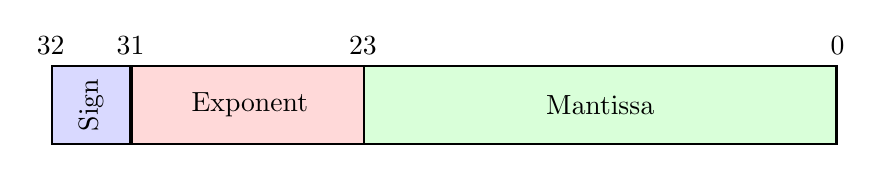
\begin{tikzpicture}[
			node distance=0.5cm,
			rect/.style={rectangle, draw, thick, minimum size=7mm}
			]
			
			\node[rect] (sign) [fill=blue!15, rotate=90,minimum width=1cm,minimum height=1cm] {Sign};
			\node[rect] (exp) [right=5mm, fill=red!15,minimum width=3cm,minimum height=1cm] {Exponent};
			\node[rect] (mant) [right=3.45cm, fill=green!15,minimum width=6cm,minimum height=1cm] {Mantissa};
			\node [above] at (mant.north east) {0};
			\node [above] at (mant.north west) {23};
			\node [above] at (exp.north west) {31};
			\node [above] at (sign.north east) {32};
		\end{tikzpicture}
	\end{figure}
	
	\begin{itemize}
		\item First bit denotes the sign $ s $ of the number
		\item Second field is the exponent $ e $ of the number
		\item Third field is the mantissa $ m $ of the number, it contains the fractional part of the number in normalized binary form
	\end{itemize}
	Thus the floating-point value is encoded and calculated as 
	\[
		(-1)^s 2^{e-bias} (1+m)
	\]
	Floating point numbers are fundamentally imprecise because they represent fractional values with a finite number of bits.

	
	\section{Objects, Values, and Types}
	
	The meaning of bits in memory is completely dependent on the \textit{type} used to access it.\\
	
	Some terminology:
	
	\begin{itemize}
		\item Type: Defines a set of possible values and a set of operations for an object.
		\item Object: Memory that holds a value of a given type.
		\item Value: Set of bits in memory interpreted according to type.
		\item Variable: Named object.
		\item Declaration: Statement that gives a name to an object.
		\item Definition: Declaration that sets aside memory for an object.
	\end{itemize}
	
	\textbf{Primitive Built-In Types}
	
	\begin{itemize}
		\item Boolean (\verb|bool|): logical values
		\item Character (\verb|char|): characters
		\item Integer (\verb|int|): integer values
		\item Floating-Point (\verb|double|): floating-point values
	\end{itemize}
	
	\subsection{Boolean}
	
	The possible values of a boolean are true or false.\\
	
	In both arithmetic and logical expressions:
	\begin{itemize}
		\item Bools are converted to integers
		\item Arithmetic and/or logical operations are performed on the converted values
		\item If the result is converted back to bool, a nonzero value is converted to true whereas a zero value to false
		\item True has the value 1, false has the value 0.
	\end{itemize}

	\subsection{Character}
	
	Can hold a character of the implementation's character set. Each character constant has an integer value; however, whether char is signed or unsigned is implementation-defined. Chars are also integral types, so arithmetic and logical operations apply.\\
	
	\textbf{Character Literal}: Notation for representing a fixed value. Also known as character constants. Enclosed by single quotes.
	
	\begin{center}
		\verb|char| ch = `A';
	\end{center}
	
	\subsection{Integer}
	
	Three integer types that vary size:
	\begin{itemize}
		\item \verb|short int|
		\item plain \verb|int|
		\item \verb|long int|
	\end{itemize}
	
	Plain integers are always signed. \\
	
	\textbf{Integer Literals}: Decimal, octal, hexidecimal, character literals.
	
	\subsection{Floating-Point}
	
	Three floating-point types that vary in size:
	\begin{itemize}
		\item \verb|float| (single-precision)
		\item \verb|double| (double-precision)
		\item \verb|long double| (extended-precision)
	\end{itemize}

	The default floating-point type is \verb|double|.
	
	\subsection{Variables}
	
	A program variable is an abstraction of a computer memory cell or collection of program cells. A variable can be characterized as a sextuple of attributes:
	\begin{itemize}
		\item Name
		\item Address
		\item Value
		\item Type
		\item Lifetime
		\item Scope
	\end{itemize}
	
	\subsubsection*{Name}
	
	Composed of a sequence of letters/characters. The first character in the name must be a letter. Keywords such as \verb|return| or \verb|string| cannot be used as variable names.
	
	\subsubsection*{Address}
	
	The machine memory address with which the variable is associated. It is possible to have multiple names with the same address (aliases).
	
	\subsubsection*{Value}
	
	The contents of the memory cell(s) associated with the variable. It appears on the right side of the assignment statement.
	
	\subsubsection*{Type}
	
	Determines the range of values the variable can store and the set of operations that are defined for the values of that type.
	
	\subsubsection*{Lifetime}
	
	The time during which the variable is bound to a specific memory location (allocation). Begins when the variable is bound to a specific cell. Ends when the variable is unbound from that cell.
	
	\subsubsection*{Scope}
	
	Part of the program in which a name has a particular meaning. Names are visible from the point where they are declared to the end of the scope in which their declaration disappears.
	
	\subsection{Declarations}
	
	Each named object has a specific type associated with it, which determines the values put in it. Before a name can be used, we inform the compiler of its type through \textit{declarations}. Most declarations are definitions, especially for arithmetic types. There must always be one definition for each name entity.
	
	
	\section{Expressions and Statements}
	
	\textbf{Statement}: A complete and meaningful command that can be given to a computer. In C++, a semicolon denotes the end of a statement.\\
	
	\textbf{Unary Operator}: Acts on 1 operand $ (++,--) $
	
	\textbf{Binary Operator}: Acts on 2 operands $ (+,-,*,\div) $
	
	\subsection{If Statement}
	
	Conditionally executes another statement based on whether a specified condition is true.
	
	\begin{minipage}[t]{.45\textwidth}
		\begin{lstlisting}[gobble=12]
		if (condition)
			statement
		\end{lstlisting}
	\end{minipage}\hfill
	\begin{minipage}[t]{.45\textwidth}
		\begin{lstlisting}[gobble=12]
		if (condition)
			statement
		else
			statement
		\end{lstlisting}
	\end{minipage}
	
	\textbf{Iterative Statements}: Provide for repeated execution until a condition is true.
	
	\subsection{While Statement}
	
	Repeatedly executes a statement as long as a condition is true.
	

	\begin{lstlisting}[gobble=8]
			while (condition)
				statement
	\end{lstlisting}

	For example, these are used when reading an input from the user.
	
	\subsection{For Statement}
	
	\begin{lstlisting}[gobble=16]
			for (init-statement; condition; expression)
				statement
	\end{lstlisting}

	\subsection{Do-While}
	
	The loop body is executed at least once, regardless of the value of the condition.
	\begin{lstlisting}[gobble=8]
			do
				statement
			while (condition)
	\end{lstlisting}

	\subsection{Debugging}
	
	Always write readable code (comment!)
	\begin{itemize}
		\item Use meaningful names
		\item Indent
		\item Use consistent layout
	\end{itemize}
	Break code into small functions
	
	
	\section{Compound Types, Compound Data}
	
	\textbf{Compound Type}: Defined in terms of another type.
	
	\subsection{References}
	
	Creates an alias for an object, allowing indirect access to that object.
	\begin{lstlisting}[gobble=4]
			int i = 11;
			int &r = i;
	\end{lstlisting}
	So \verb|i| and \verb|r| refer to the same object (11).\\
	
	A reference is another name for an already existing object.
	
	\subsection{Pointers}
	
	Compound data type that ``points" to another type.
	
	\subsection{Array}
	
	Sequence of objects allocated in contiguous memory (all same type).
	\begin{lstlisting}[gobble=4]
			int arr[7];
	\end{lstlisting}
	This creates an array named \verb|arr| that has 8 \verb|int| objects.
	
	\subsection{Vector}
	
	Like arrays, but can hold an arbitrary number of objects. You can add objects to vectors with \verb|push_back()|.
	
	\section{Type Conversions}
	
	\subsection{Narrowing Conversions}
	
	Converts a value to a type that cannot store even approximations of all the values of the original type. For example, converting a \verb|double| to a \verb|float|.
	
	\subsection{Widening Conversions}
	
	Converts a value to a type that can include at least approximations of all of the values of the original type. For example, \verb|int| to \verb|double|.\\
	
	Narrowing conversions aren't always safe whereas widening conversions are almost always safe.\\
	
	\textbf{Coercion}: Implicit type conversion that is initiated by the compiler or runtime system.\\
	
	\textbf{Explicit Type Conversions}: Casts. Use the command
	\begin{lstlisting}[gobble=12]
			static_cast<type> (value to cast)
	\end{lstlisting}	
	Helpful for say floating-point division between two integers.
	
	\begin{center}
		\begin{tabular}{c|c}
			   Safe Type Conversions       &   Unsafe Type Conversions     \\ \hline
			 \verb|bool| to \verb|char|    &  \verb|double| to \verb|int|  \\
			 \verb|bool| to \verb|int|     &  \verb|double| to \verb|char| \\
			 \verb|bool| to \verb|double|  &  \verb|double| to \verb|bool| \\
			 \verb|char| to \verb|int|     &  \verb|int|    to \verb|char| \\
			 \verb|char| to \verb|double|  &  \verb|int|    to \verb|bool| \\
			 \verb|int|  to \verb|double|  &  \verb|char|   to \verb|bool|
		\end{tabular}
	\end{center}
	
	\section{Errors}
	
	\subsection{Compile Time Errors}
	
	\begin{itemize}
		\item Syntax errors
		\item Type errors
	\end{itemize}

	\subsection{Link Time Errors}
	
	Error found by linker when trying to combine object files into an executable, e.g an undefined function.
	
	\subsection{Run-Time Errors}
	
	Errors found by checks made during a running program
	\begin{itemize}
		\item The computer (hardware)
		\item A library
		\item User code (divide by zero)
	\end{itemize}

	\subsection{Logic Errors}
	
	Found by the programmer looking for the causes of erroneous results.
	
	\section{I/O Streams}
	
	\textbf{Stream}: A programming language construct that provides you with a character based interface to I/O devices.\\
	
	\textbf{Stream Buffer}: Houses a fixed amount of extracted stream data.
	
	\subsection{OStream}
	
	Turns values of various types into character sequences, sends them somewhere. The command \verb|std::cout| is an ostream typed object that provides character sequences to standard output.
	
	\subsection{IStream}
	
	Turns character sequences into values of various types, gets those characters from somewhere. The command \verb|std::cin| is an istream typed object that consumes character sequences from standard input.
	
	\subsection{The I/O Classes}
	
	 \begin{itemize}
	 	\item IOStream
	 		\begin{itemize}
	 			\item \verb|istream| reads from a stream
	 			\item \verb|ostream| writes to a stream
	 		\end{itemize}
 		\item FStream
 			\begin{itemize}
 				\item \verb|ifstream| reads from a file
 				\item \verb|ofstream| writes a file
 				\item \verb|fstream| reads and writes a file
 			\end{itemize}
 		\item Sstream
 			\begin{itemize}
 				\item \verb|istringstream| reads from a string
 				\item \verb|ostringstream| writes a string
 				\item \verb|stringstream| reads and writes a string
 			\end{itemize}
	 \end{itemize}
 
 	\textbf{General Model}
 	
 	\begin{center}
 		\begin{tikzpicture}[
 			node distance=0.5cm,
 			rect/.style={rectangle, draw, fill=blue!15, thick, minimum size=7mm}
 		]
 		\node [thick, double arrow,draw, fill=red!15, text width=2.5cm,align=center] (IO) {I/O System};
 		\node[rect] (main) [right= of IO] {Main memory};
 		\node[thick, cylinder, shape border rotate=90, draw, fill=green!15,aspect=0.5,minimum height=1.5cm,minimum width=1.5cm, align=center, left= of IO] (disk) {Disk};
 		\node [below= of disk] {Files};
 		\node [below= of IO] {IOStreams};
 		\node [below= of main] {Objects};
 		\end{tikzpicture}
 	\end{center}
	
	To read a file, we must:
	\begin{itemize}
		\item Know its name
		\item Open it for reading
		\item Ensure that it opened successfully 
		\item Read it
		\item Close it
	\end{itemize}

	To write a file, we must:
	\begin{itemize}
		\item Know its name
		\item Open it for writing
		\item Ensure that it opened successfully
		\item Write to it
		\item Close it
	\end{itemize}
	
	To construct an ifstream and open a file, we write
	\begin{lstlisting}[gobble=4]
		ifstream in(file);
	\end{lstlisting}
	To construct an ofstream, we write
	\begin{lstlisting}[gobble=4]
		ofstream out(file);
	\end{lstlisting}
	
	\subsection{Stream State Flags}
	
	The I/O stream types each provide a collection of bits that are used to convey information about the state of a stream.
	\begin{itemize}
		\item \verb|goodbit|: Set when the stream is not in an error state
		\item \verb|badbit|: Set when an unrecoverable failure has occurred 
		\item \verb|failbit|: Set when a recoverable error has occurred
		\item \verb|eofbit|: Set when the stream has hit the end of the file
	\end{itemize}
	
	\section{Function Basics}
	
	\subsection{Function Declarations}
	
	We can declare a function by writing a declaration of the form \verb|f(args)|, where \verb|f| is the name being introduced and \verb|args| is a list of zero or more parameters.
	\begin{lstlisting}[gobble=4]
		double mult(double, double);
	\end{lstlisting}
	The base type specifies the return type. Put \verb|void| if you don't want to return anything.
	
	\subsection{Function Definition}
	
	A declaration that fully specifies the entity being declared
	\begin{lstlisting}[gobble=4]
		double mult(double x, double y) {
		    return x*y;
		}
	\end{lstlisting}
	A declaration introduces a name to the compiler and how that name can be used. A \textit{header file} is a file containing declarations, these files end with the extension \verb|.h|. Header guards make up the \verb|.h| file:
	\begin{lstlisting}[gobble=4]
		#ifndef DESCRIPTIVE_NAME_H
		#define DESCRIPTIVE_NAME_H
		// function declarations go here
		#endif
	\end{lstlisting}
	These correspond to the file \verb|descriptive_name.h|. We would then write a \verb|descriptive_name.cpp| that contains our function definitions. Then we can use these new functions in \verb|main.cpp| by writing \verb|#include "descriptive_name.h"| in the header.\\
	
	If done wrong, this would result in a linker error.
	
	
	\section{Function Argument Passing}
	
	\textbf{Pass-by-Value}: A value is copied into an object for initialization.
	
	\textbf{Pass-by-Reference}: The parameter binds to the object being passed: the parameter becomes an alias for the object to which it is bound.
	
	\subsection{Pass-by-Value}
	
	Working with a copy of the argument
	
	\subsection{Pass-by-Reference}
	
	Changes that the function ``makes" on a reference parameter will always be reflected in the object bound to that reference. The reference parameter is simply another name for the object for which it is initialized.\\
	
	Pass large objects by reference to avoid copying large arguments.\\
	
	Used to return multiple objects in functions.
	
	\subsection{Pass-by-Constant-Reference}
	
	Used when passing large objects and want the benefit of pass-by-reference, but d not need to modify arguments.
	
	\subsection{Guidance for Passing Arguments}
	
	\begin{itemize}
		\item Use pass-by-value for small objects (primitive data types)
		\item Use pass-by-const-reference for large objects (vectors)
	\end{itemize}

	Never return a reference or pointer to a local variable, problems will occur.
	
	\section{Functions and the Stack}
	
	The stack manages function calls that are made during executions. Each time a function is called, an \textit{activation record} for that function is pushed (added) to the stack.\\
	
	Activation records store:
	\begin{itemize}
		\item Return location
		\item Arguments passed to the function
		\item Local variables defined in the function
	\end{itemize}
	When the function returns, its activation record is popped (removed) from the stack.\\
	
	Code defining each function is stored in the code/static region of the program's address space.
	
	\section{Recursive Functions}
	
	\textbf{Recursive Function}: A function that is defined in terms of itself.\\
	
	For example, the factorial function.
	\[
		n! = \begin{cases} 1 \hspace{1.57cm} \text{ if } n < 2 \\ n \cdot (n-1)! \; \text{ if } n>2 \end{cases}
	\]
	The base case is the non recursive case. For the factorial function, the base case is when $ n<2 $.
	
	\subsection{Recursive Function and the Stack}
	
	To better illustrate what's going on, we use these function trees. For example, say we have a function called \verb|fact()| that computes the factorial. The function tree for \verb|fact(3)| looks like
	
	\begin{center}
		\begin{tikzpicture}[node distance=0.5 cm,
		rect/.style={rectangle, draw, thick, minimum size=7mm},
		]
		\node[rect] (A) [fill=red!15,minimum width=1.5cm] {caller};
		\node[rect] (B) [below= of A, fill=blue!15] {\verb|fact(3)|};
		\node[rect] (C) [below= of B, fill=blue!15] {\verb|fact(2)|};
		\node[rect] (D) [below= of C, fill=blue!15] {\verb|fact(1)|};
		
		\draw[->] (A.south) -- (B.north);
		\draw[->] (B.south) -- (C.north);
		\draw[->] (C.south) -- (D.north);
		\draw[->] (D.east) to[bend right=90] (C.east) node[below of=C, right=1.25cm] {1};
		\draw[->] (C.east) to[bend right=90] (B.east) node[below of=B, right=1.25cm] {2};
		\draw[->] (B.east) to[bend right=90] (A.east) node[below of=A, right=1.25cm] {6};
		\end{tikzpicture}
	\end{center} 
	
	The boxes represent stack frames, straight arrows are function calls, and curved arrows are return values.\\
	
	In general, anything solved recursively has an iterative solution.
	
	\section{Functions and Exceptions}
	
	\subsection{Exceptions}
	
	C++'s means of separating error reporting from error handling in a general way.\\
	
	Introduce a try block around the code where an exception might occur. Then catch the exception of a specific type.
	\begin{lstlisting}[gobble=14]
		try {
		    //stuff
		} catch (const runtime_error& e) {
		    cerr << "Exception: " << e.what() << endl;
		}
	\end{lstlisting}
	
	
	\section{Function Overloading}
	
	\textbf{Overloaded Functions}: Functions that have the same name but different parameters list and appear in the same scope.\\
	
	Eliminates the need to defined different names for different functions that perform the same general action but on different parameter types.\\
	
	\textbf{Overload Resolution}: The process by which the compiler determines which specific function is called from a set of overloaded functions. \vspace{-1mm}
	\begin{itemize}
		\item The compiler determines this by comparing the arguments against the parameters of each function in the set of overloaded functions.
	\end{itemize}

	Use function overloading when a name is semantically significant amongst different data types.\\
	
	When we overload functions, we are creating multiple functions that have the: \vspace{-1mm}
	\begin{itemize}
		\item Same name
		\item Different parameter configurations \vspace{-1mm}
			\begin{itemize}
				\item Number of parameters
				\item Types of parameters
				\item Order for parameter types
			\end{itemize}
	\end{itemize}
	
	
	\section{Dynamic Memory}
	
	\subsection*{Stack}
	
	The size of variables must be known at compile-time.\\
	
	A new block of memory called the stack frame (activation record) is added to the stack to hold automatic variables each time you call a method. 
	
	\subsection*{Heap/Free Store}
	
	Size of variables may be unknown at compile-time.\\
	
	Allocation is performed at run-time.\\
	
	Dynamically created objects are stored on the free store.
	
	\subsection{Allocation of Memory to Variables (stack)}
	
	When we write something like \verb|int k = 11|, when the compiler sees this, it determines the amount of memory to hold the value of an \verb|int|, and adds the identifier \verb|k| to a symbol table with its memory address in which the object will become accessible during run-time.\\
	
	When a function is called, the stack pointer is moved in one direction to allocate memory on the stack for the local variables associated with the called function.\\
	
	When the function finishes execution, the stack pointer is moved back in the other direction, and memory is deallocated.\\
	
	If the sizes of the local variables are fixed at compile-time and stored in the same order in the activation record each time the function is invoked, then the location of each variable will be a fixed offset from the stack pointer.
	
	\subsection{Dynamically Allocated Objects (heap/free store)}
	
	We dynamically allocate memory on the free store using the \verb|new| operator. \vspace{-1mm}
	\begin{itemize}
		\item The \verb|new| operator allocates memory for an object of a specified type.
		\item The \verb|new| operator returns the address of the region of memory allocated for that object.
	\end{itemize} \vspace{-1mm}
	It's our responsibility to explicitly deallocate that memory when we are finished using it; we do this by using the address as an operand to the \verb|delete| operator.
	
	\begin{center}
		\begin{tabular}{|c|c|} \hline
			\thead{\textbf{Clause}} & \thead{\textbf{Result of Violation}} \\ \hline
			\makecell[l]{You will eventually return the memory you\\ borrow} & Memory Leak \\ \hline
			\makecell[l]{You will immediately stop using that memory \\ that you've returned} & Dangling Pointer \\ \hline
			\makecell[l]{You will not return memory that you did not\\ borrow (and you will not twice return memory\\ that you've borrowed once)} & Corrupted Heap \\ \hline
		\end{tabular}
	\end{center}
	
	\textbf{Memory Leak}: Occurs when we dynamically allocate memory for an object, but fail to ever deallocate that space when we're done using it.\\
	
	\textbf{Dangling Pointer}: When a pointer to a piece of memory that has deallocated is used. Until that memory is actually allocated again, you may continue to get the value that was stored in the object that used to reside there.\\
	
	\textbf{Corrupted Heap}: Happens when something is deallocated that is not allocated.
	
	
	\section{Classes}
	
	\textbf{Class}: A user-defined type: composed of built-in types, other compositions, and functions.\\
	
	A class provides the description for how objects of that type are to be represented.
	\begin{itemize}
		\item The representation of the user-defined types is composed of built-in types and other user-defined types that are known as \textit{data members}
		\item \textit{Function members} are written to provide the operations that we will be able to apply to the objects of our user-defined type.
	\end{itemize}
	
	\subsection*{Why classes?}
	\begin{itemize}
		\item \textit{Data abstraction} allows us to focus on what operations that will be performed on the data members opposed to how we will perform those operations; hidden is underlying structure, increased is the modularity and transparency.
		\item \textit{Encapsulates} data together with the operations that can be performed on that data.
		\item \textit{Data hiding} can be accomplished using member access specifiers: restrict interaction with class members across a well-defined public interface; present only the fundamental facilities that the user needs for use, and hide all implementation details within the class itself.\\
	\end{itemize}
	
	\verb|class| members are private by default, whereas \verb|struct| members are public by default
	
	
	\subsection*{Data members: Public or Private?}
	\begin{itemize}
		\item If the value assigned to an object will work regardless, declare public.
		\item If the value assigned to an object needs to be checked, or must conform to the same requirements, declare private.
	\end{itemize}
	
	Making attributes private can help maintain the integrity of our data members by inhibiting the direct manipulation of their values; interaction with private data members are limited to the extent provided by the public interface.\\
	
	If you want private attributes to be ``public", use accessors/mutators.
	
	
	\subsection{Accessors(getters) and Mutators(setters)}
	
	\textbf{Accessor(getter)}: A function that returns the value stored in a private data member.\\
	
	\textbf{Mutator(setter)}: A function that stores a value in a private data member or mutates its state.\\
	
	Member function declarations for your class should be stored in the \verb|ClassName.h| file. Member function definitions for your class should be stored in the \verb|ClassName.cpp| file with scope resolution (e.g. \verb|ClassName::getx() {return x;}|).
	
	
	\subsection{Constructors}
	
	In order to initialize our data members upon object instantiation, we write a special member function known as the \textit{constructor}.
	\begin{itemize}
		\item The \textit{constructor} is implicitly invoked whenever an object of the user-defined type is created.
			\begin{itemize}
				\item Its job is to construct an object and do initialization if necessary
			\end{itemize}
		\item We can also acquire resources in the constructor; maybe allocate dynamic memory for some object, or open a file
	\end{itemize}

	We can overload constructors of a user-defined type; we typically use \textit{parameterized constructors} to initialize data members.
	
	\subsection*{Destructors}
	
	Much like how a constructor is called whenever an object of a user-defined type is created, a \textit{destructor} is called when an object's lifetime is up.
	\begin{itemize}
		\item One primary use for a destructor is to release resources that the object had required during construction.
	\end{itemize}

	There is only one destructor per class(can't be overloaded).
	
	
	\section{Overloaded Operators for User-Defined Types}
	
	An overloaded operator has the same number of parameters as the operator has operands (single parameter for unary, two parameters for binary).
	\begin{itemize}
		\item For binary, the left-hand argument is used to initialize the first parameter and the right-hand argument the second.
	\end{itemize}
	
	We can only overload existing operators: can't invent new operator symbols.\\
	
	If the overloaded operator is defined as a member function, the first operand is bound to the implicit \verb|this| pointer.
	\begin{itemize}
		\item Due to this, a member operator function will have one less (explicit) parameter than the operator has operands.
	\end{itemize}

	If the overloaded operator is defined as a non-member function, at least one of its parameters must be a user-defined type
	\begin{itemize}
		\item This implies that we cannot change the meaning of an operator when applied to operands of built-in type.
	\end{itemize}


	



	
	
	
	
	
	
	
	
	
	
	
	
	
	
\end{document}